\documentclass[12pt]{beamer}
\newenvironment{ConCodigo}[1]
  {\begin{frame}[fragile,environment=ConCodigo]{#1}}
  {\end{frame}}
\graphicspath{{Imagenes/}{../Imagenes/}}
\usepackage[utf8]{inputenc}
\usepackage[spanish]{babel}
\usepackage{hyperref}
\usepackage{etex}
\reserveinserts{28}
\usepackage{amsmath}
\usepackage{amsthm}
\usepackage{mathtools}
\usepackage{multicol}
\usepackage{multirow}
\usepackage{tabulary}
\usepackage{booktabs}
\usepackage{nccmath}
\usepackage{biblatex}
\usepackage{epstopdf}
\usepackage{graphicx}
%\usepackage{enumitem,xcolor}
\usepackage{siunitx}
\sisetup{scientific-notation=true}
%\usepackage{fontspec}
\usepackage{lmodern}
\usepackage{float}
\usepackage[format=hang, font=footnotesize, labelformat=parens]{caption}
\usepackage[autostyle,spanish=mexican]{csquotes}
\usepackage{standalone}
\usepackage{blkarray}
\usepackage{algorithm}
\usepackage{algorithmic}
\usepackage{tikz}
\usepackage[siunitx]{circuitikz}
\usetikzlibrary{arrows,patterns,shapes}
\usetikzlibrary{decorations.markings}
\usetikzlibrary{arrows}
\usepackage{color}
\usepackage{xcolor}
%\usepackage{beton}
%\usepackage{euler}
%\usepackage[T1]{fontenc}
\usepackage[sfdefault]{roboto}  %% Option 'sfdefault' only if the base font of the document is to be sans serif
\usepackage[T1]{fontenc}
\renewcommand*\familydefault{\sfdefault}
\DeclareGraphicsExtensions{.pdf,.png,.jpg}
\usepackage{hyperref}
\renewcommand {\arraystretch}{1.5}
\newcommand{\python}{\texttt{python}}
\usefonttheme[onlymath]{serif}
\setbeamertemplate{navigation symbols}{}
\usetikzlibrary{patterns}
\usetikzlibrary{decorations.markings}
\tikzstyle{every picture}+=[remember picture,baseline]
%\tikzstyle{every node}+=[inner sep=0pt,anchor=base,
%minimum width=2.2cm,align=center,text depth=.15ex,outer sep=1.5pt]
%\tikzstyle{every path}+=[thick, rounded corners]
\setbeamertemplate{caption}[numbered]
\newcommand{\ptm}{\fontfamily{ptm}\selectfont}
%Se usa la plantilla Warsaw modificada con spruce
\mode<presentation>
{
  \usetheme{Warsaw}
  \setbeamertemplate{headline}{}
  \useoutertheme{default}
  \usecolortheme{seahorse}
  \setbeamercovered{invisible}
}
% \AtBeginSection[]
% {
% \begin{frame}<beamer>{Contenido}
% \normalfont\mdseries
% \tableofcontents[currentsection]
% \end{frame}
%}

\usepackage{listings}
\lstset{ %
language=Python,                % choose the language of the code
basicstyle=\small,       % the size of the fonts that are used for the code
numbers=left,                   % where to put the line-numbers
numberstyle=\footnotesize,      % the size of the fonts that are used for the line-numbers
stepnumber=1,                   % the step between two line-numbers. If it is 1 each line will be numbered
numbersep=5pt,                  % how far the line-numbers are from the code
backgroundcolor=\color{white},  % choose the background color. You must add \usepackage{color}
showspaces=false,               % show spaces adding particular underscores
showstringspaces=false,         % underline spaces within strings
showtabs=false,                 % show tabs within strings adding particular underscores
frame=single,   		% adds a frame around the code
tabsize=4,  		% sets default tabsize to 2 spaces
captionpos=b,   		% sets the caption-position to bottom
breaklines=true,    	% sets automatic line breaking
breakatwhitespace=false,    % sets if automatic breaks should only happen at whitespace
escapeinside={\#}{)}          % if you want to add a comment within your code
}

\begin{document}
\title{Examen 3 - Ecuaciones Diferenciales Ordinarias}
\subtitle{Soluci\'{o}n}
%\subsubtitle{Curso de F\'{i}sica Computacional}
\author{M. en C. Gustavo Contreras May\'{e}n}
%\email{curso.fisica.comp@gmail.com}
%\ptsize{10}
\maketitle
\fontsize{14}{14}\selectfont
\spanishdecimal{.}
\begin{frame}{Contenido}
\tableofcontents[pausesections]
\end{frame}
\section{Problema 1}
\begin{frame}[fragile]
\frametitle{Problema 1}
La ecuaci\'{o}n diferencial del movimiento de un p\'{e}ndulo simple es
\[ \dfrac{d^{2} \theta}{d t^{2}} = - \dfrac{g}{L} \sin \theta \]
donde
$\theta$ es el desplazamiento angular a partir de la vertical, $g$ es la aceleraci\'{o}n debida a la gravedad y $L$ la longitud del p\'{e}ndulo.
\end{frame}
\begin{frame}
Con el cambio de variable $\tau = t \sqrt{g/L}$, la ecuaci\'{o}n toma la forma:
\[ \dfrac{d^{2} \theta}{d \tau^{2}} = -  \sin \theta\]
Resuelve la ecuaci\'{o}n para determinar el per\'{i}odo del p\'{e}ndulo, si la amplitud es $\theta_{0} = 1$ rad. Considera que para pequeñas amplitudes ($\sin \theta \simeq \theta$) el per\'{i}odo es $2 \pi \sqrt{L/g}$.
\end{frame}
\begin{frame}[fragile]
\frametitle{Soluci\'{o}n}
El sistema de 1-EDO que resulta es:
\begin{lstlisting}
def F(x,y):
    F=zeros((2), dtype="float64")
    F[0]=y[1]
    F[1]=-sin(y[0])
    return F

x=0.0
xAlto=20
y=array([1.0,0.0])
h=0.1
freq=5

X,Y=integra(F,x,y,xAlto,h)
\end{lstlisting}
\end{frame}
\begin{frame}[fragile]
\frametitle{Gr\'{a}fica de la soluci\'{o}n}
\begin{figure}
	\centering
	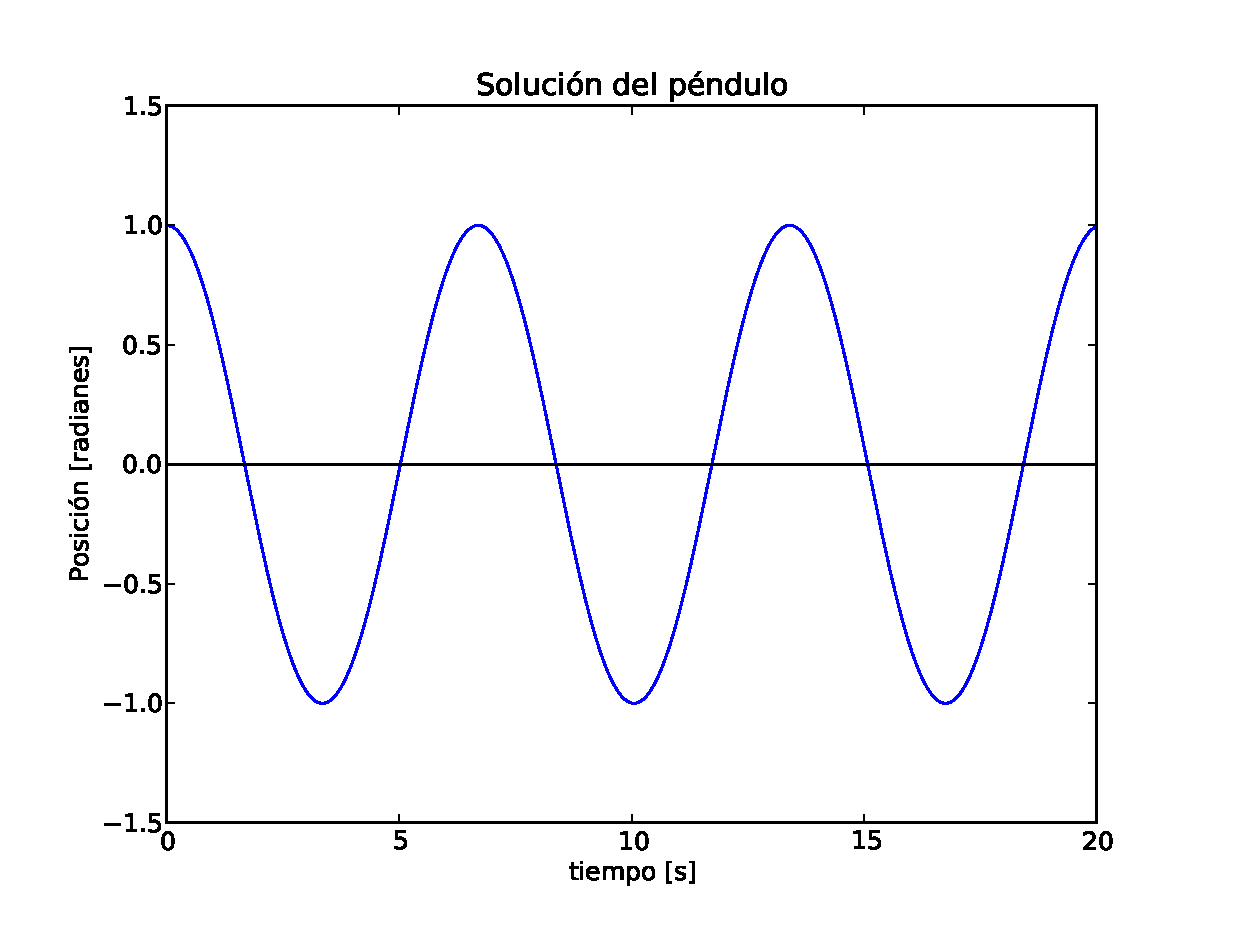
\includegraphics[scale=0.5]{Problema1_01.eps} 
\end{figure}
\end{frame}
\begin{frame}
\frametitle{C\'{a}lculo del per\'{i}odo}
Sabemos de la tema anterior de integraci\'{o}n que el per\'{i}odo de un p\'{e}ndulo de longitud $L$ es $\tau = 4 \sqrt{\frac{L}{g}} h(\theta_{0})$, donde $g$ es la aceleraci\'{o}n debida a la gravedad, $\theta_{0}$, representa la amplitud angular y 
\[ h(\theta_{0}) =  \int_{0}^{\frac{\pi}{2}} \dfrac{d\theta}{\sqrt{1 - \sin^{2} \left( \frac{\theta_{0}}{2}\right) \sin^{2} \theta}} \]
\end{frame}
\begin{frame}

\end{frame}
\end{document}